\begin{enumerate}
	\item Exercício
	
	\begin{equation*}
		R = \left\{(x, y) \in \mathbb{R}^2 \,|\, 0 \leq x \leq 2 \,,\, 0 \leq y \leq 6 \right\}	
	\end{equation*}
	
	\begin{figure}[htb]
		\caption{Integrais duplas - Aula 2 - Exercício I}
		\label{v02_a02_e01}
		\centering
		
\includegraphics[width=0.5\textwidth]{v02_a02_e01.png}		
	\end{figure}
	
	\begin{gather*}
		a = \int_0^2 dx \int_0^6 dy = \int_0^2 dx\, [y]_0^6 = \int_0^2 dx\, [6 - 0] = 6\int_0^2 dx = 6[x]_0^2 =\\ 6[2 - 0] = 6 \cdot 2 = 12
	\end{gather*}
		
	\item Exercício
	
	\begin{equation*}
		R = \left\{(x, y) \in \mathbb{R}^2 \,|\, 0 \leq x \leq 1 \,,\, x \leq y \leq 2x \right\}
	\end{equation*}
							
	\begin{figure}[htb]
		\caption{Integrais duplas - Aula 2 - Exercício II}
		\label{v02_a02_e02}
		\centering
		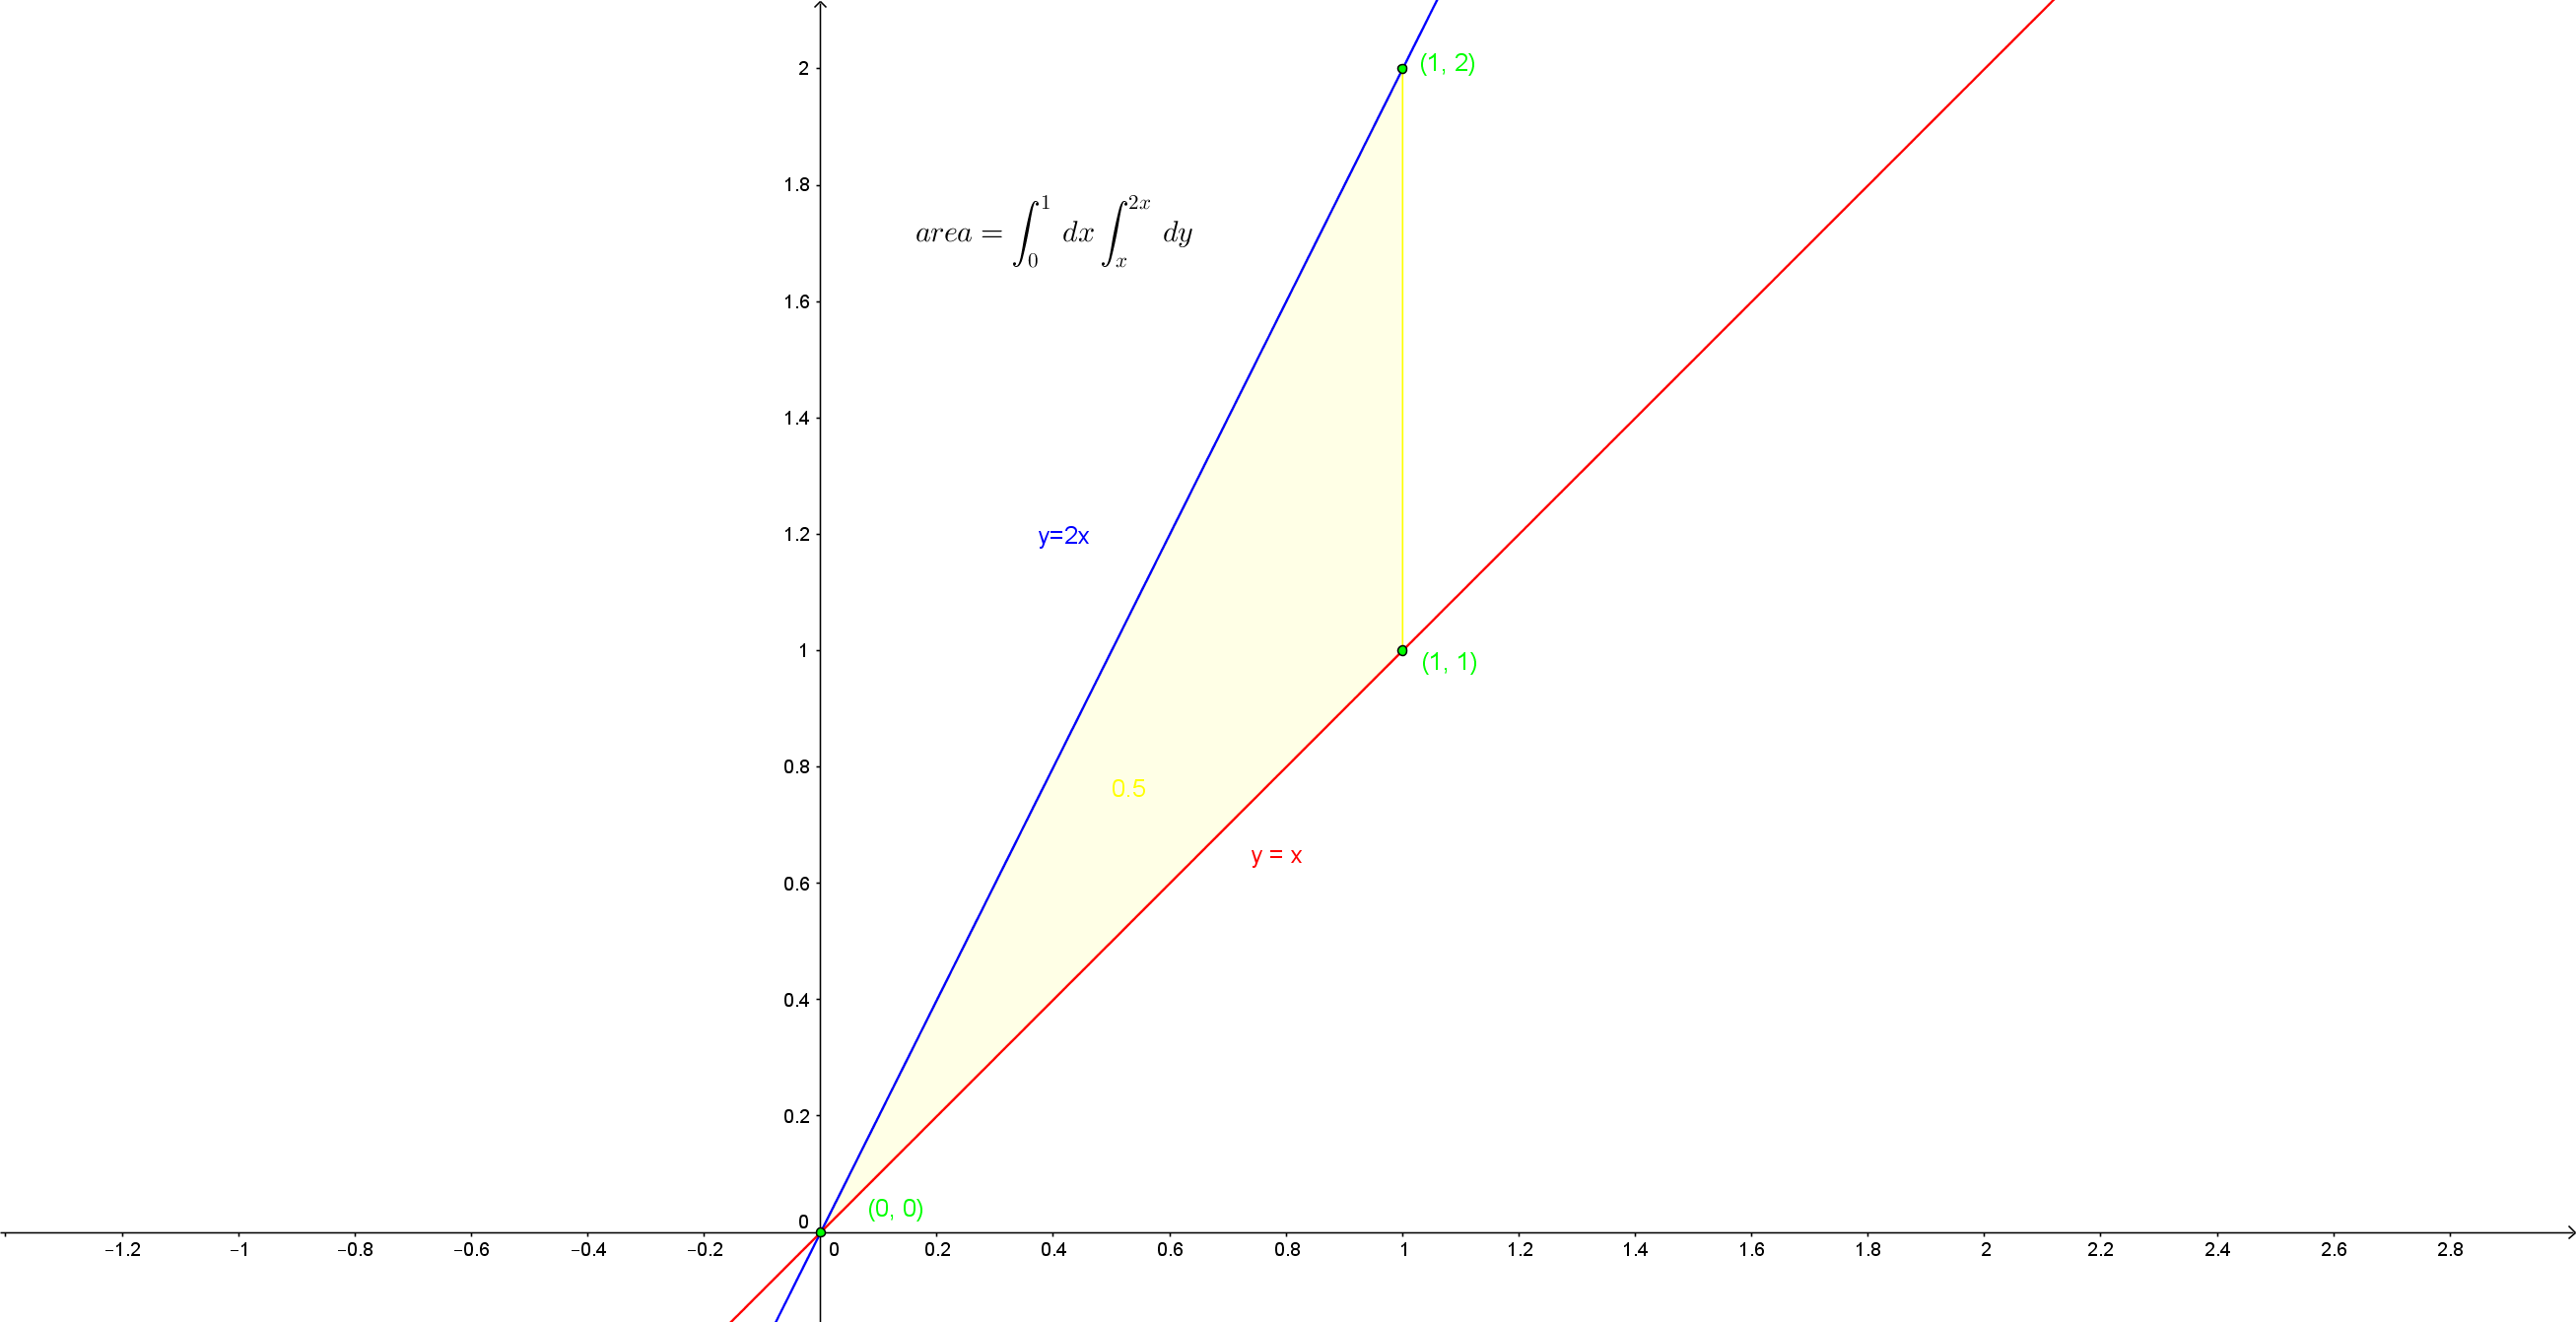
\includegraphics[width=0.5\textwidth]{v02_a02_e02.png}		
	\end{figure}
	
	\begin{gather*}
		a = \int_0^1 dx \int_{x}^{2x} dy = \int_0^1 dx\, [y]_{x}^{2x} = \int_0^1 dx\, [2x - x] = 2\int_0^1 x\, dx - \int_0^1 x\, dx =\\ \left[\overstrike{2}\dfrac{x^2}{\overstrike{2}} - \dfrac{x^2}{2}\right]_0^1 = \left[\dfrac{2x^2 - x^2}{2}\right]_0^1 = \dfrac{1}{2}\left[x^2\right]_0^1 = \dfrac{1}{2}\left[1^2 \overstrike{- 0^2}\right] = \dfrac{1}{2} = 0,5
	\end{gather*}
		
	\item Exercício
	
	\begin{equation*}
		R = \left\{(x, y) \in \mathbb{R}^2 \,|\, 0 \leq y \leq 1 \,,\, 0 \leq x \leq \sqrt{1 - y^2} \right\}
	\end{equation*}
	\begin{equation*}
		y = 0,\, y = 1
	\end{equation*}
	\begin{equation*}
		x = 0,\, x = \sqrt{1 - y^2} \Rightarrow x^2 = 1 - y^2 \Rightarrow x^2 - 1 = -y^2 \Rightarrow y^2 = -x^2 + 1 \Rightarrow y = \sqrt{1 -x^2}
	\end{equation*}
					
	\begin{figure}[htb]
		\caption{Integrais duplas - Aula 2 - Exercício III}
		\label{v02_a02_e03}
		\centering
		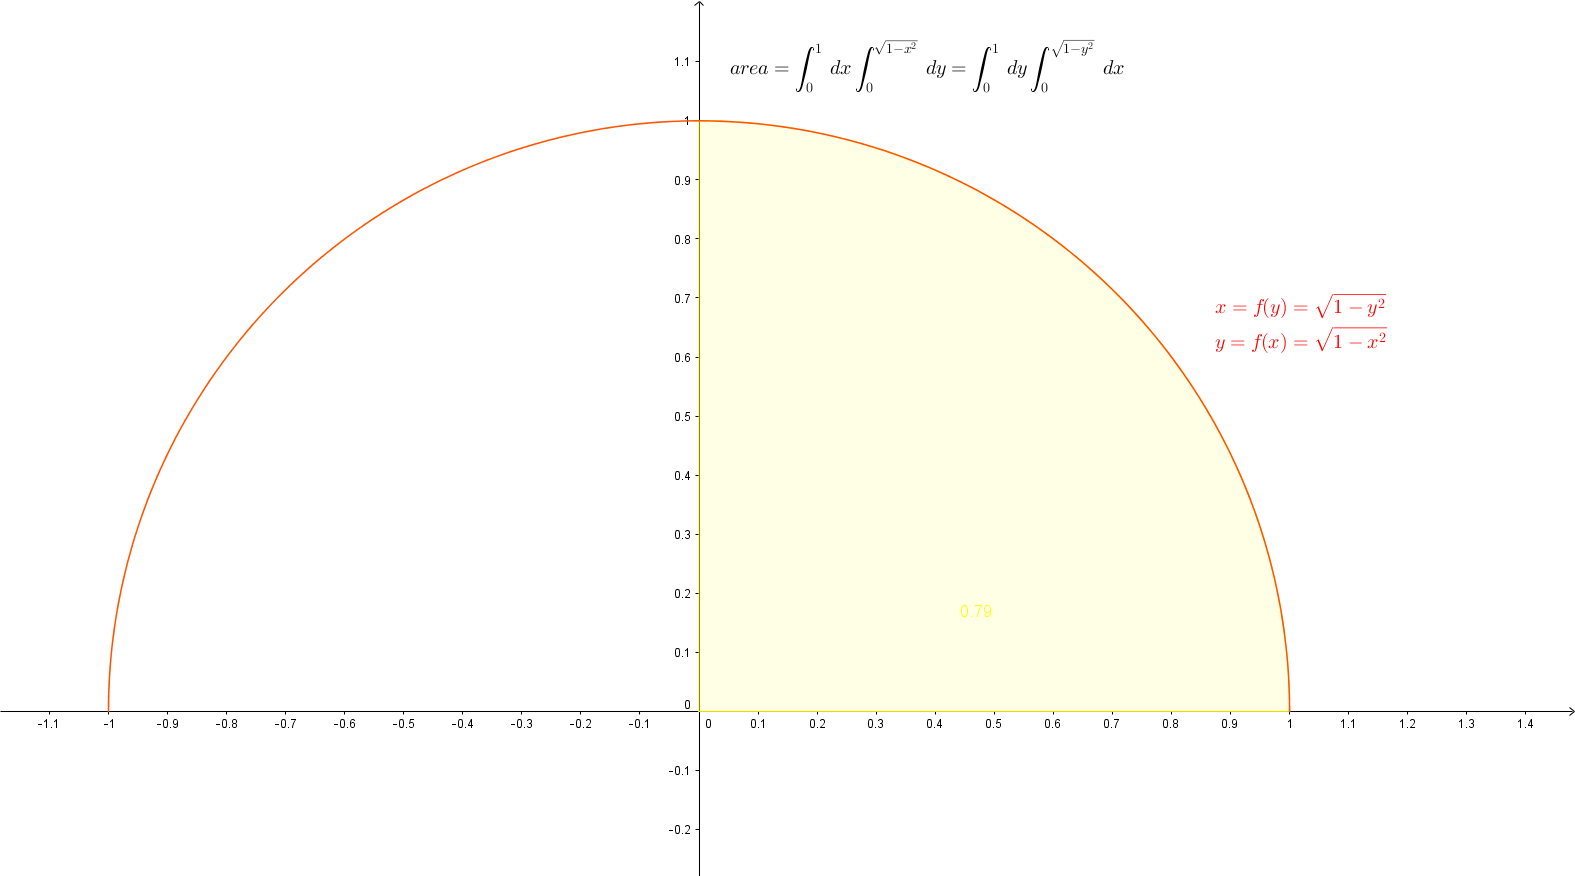
\includegraphics[width=0.5\textwidth]{v02_a02_e03.png}		
	\end{figure}
	
	\begin{gather*}
		a = \int_0^1 dy \int_0^{f(y)} dx = \int_0^1 dy \int_0^{\sqrt{1 - y^2}} dx = \int_0^1 dy\, [x]_0^{\sqrt{1 - y^2}} = \int_0^1 dy\, \left[\sqrt{1 - y^2} - 0\right] =\\ \int_0^1 \sqrt{1 - y^2}\, dy = \int_0^1 \sqrt{1 - \sen^2(t)}\, \cos(t) dt = \int_0^1 \sqrt{\cos^2(t)}\, \cos(t) dt =\\ \int_0^1 \cos(t)\cos(t) dt = \int_0^1 \cos^2(t) dt = \int_0^1 \dfrac{1 + \cos(2t)}{2} dt = \dfrac{1}{2}\int_0^1 \left[1 + \cos(2t)\right] dt =\\ \dfrac{1}{2}\int_0^1 dt + \dfrac{1}{2}\int_0^1 \cos(2t) dt = \dfrac{1}{2}\int_0^1 dt + \dfrac{1}{2}\int_0^1 \cos(u) \dfrac{du}{2} = \dfrac{1}{2}\int_0^1 dt + \dfrac{1}{4}\int_0^1 \cos(u)\, du =\\ \left[\dfrac{1}{2}t + \dfrac{1}{4}\sen(u)\right]_0^1 = \left[\dfrac{t}{2} + \dfrac{\sen(2t)}{4}\right]_0^1 = \left[\dfrac{t}{2} + \dfrac{2\sen(t)\cos(t)}{4}\right]_0^1 = \left[\dfrac{t + \sen(t)\cos(t)}{2}\right]_0^1 =\\ \dfrac{1}{2}\left[\arcsen(y) + y\sqrt{1 - y^2}\right]_0^1 = \dfrac{1}{2}\left[\left(\arcsen(1) \overstrike{+ 1 \cdot\sqrt{1 - 1^2}}\right) - \left(\arcsen(0) \overstrike{+ 0 \cdot \sqrt{1 - 0^2}}\right)\right] =\\ \dfrac{1}{2}\left[\dfrac{\pi}{2} - 0\right] = \dfrac{\pi}{4} = 0,785
	\end{gather*}
		
	\begin{equation*}
		y = \sen(t) \Rightarrow dy = \cos(t) dt
	\end{equation*}	
	\begin{equation*}
		u = 2t \Rightarrow \dfrac{du}{2} = dt
	\end{equation*}
	\begin{equation*}
		\sen(t) = \dfrac{co}{h} = \dfrac{y}{1} = y
	\end{equation*}
	\begin{equation*}
		h^2 = co^2 + ca^2 \Rightarrow 1 = y^2 + ca^2 \Rightarrow ca = \sqrt{1 - y^2}
	\end{equation*}
	\begin{equation*}
		\cos(t) = \dfrac{ca}{h} = \dfrac{\sqrt{1 - y^2}}{1} = \sqrt{1 - y^2}
	\end{equation*}
	\begin{equation*}
		y = \sen(t) \Rightarrow t = \arcsen(y)
	\end{equation*}
			
	\item Exercício
	
	\begin{equation*}
		y = x^2 + 1 ,\, y = -x^2 - 1 ;\; x = 1 ,\, x = -1
	\end{equation*}
	\begin{equation*}
		R = \left\{(x, y) \in \mathbb{R}^2 \,|\, -1 \leq x \leq 1 \,,\, -x^2 - 1 \leq y \leq x^2 + 1 \right\}
	\end{equation*}	
	\begin{figure}[htb]
		\caption{Integrais duplas - Aula 2 - Exercício IV}
		\label{v02_a02_e04}
		\centering
		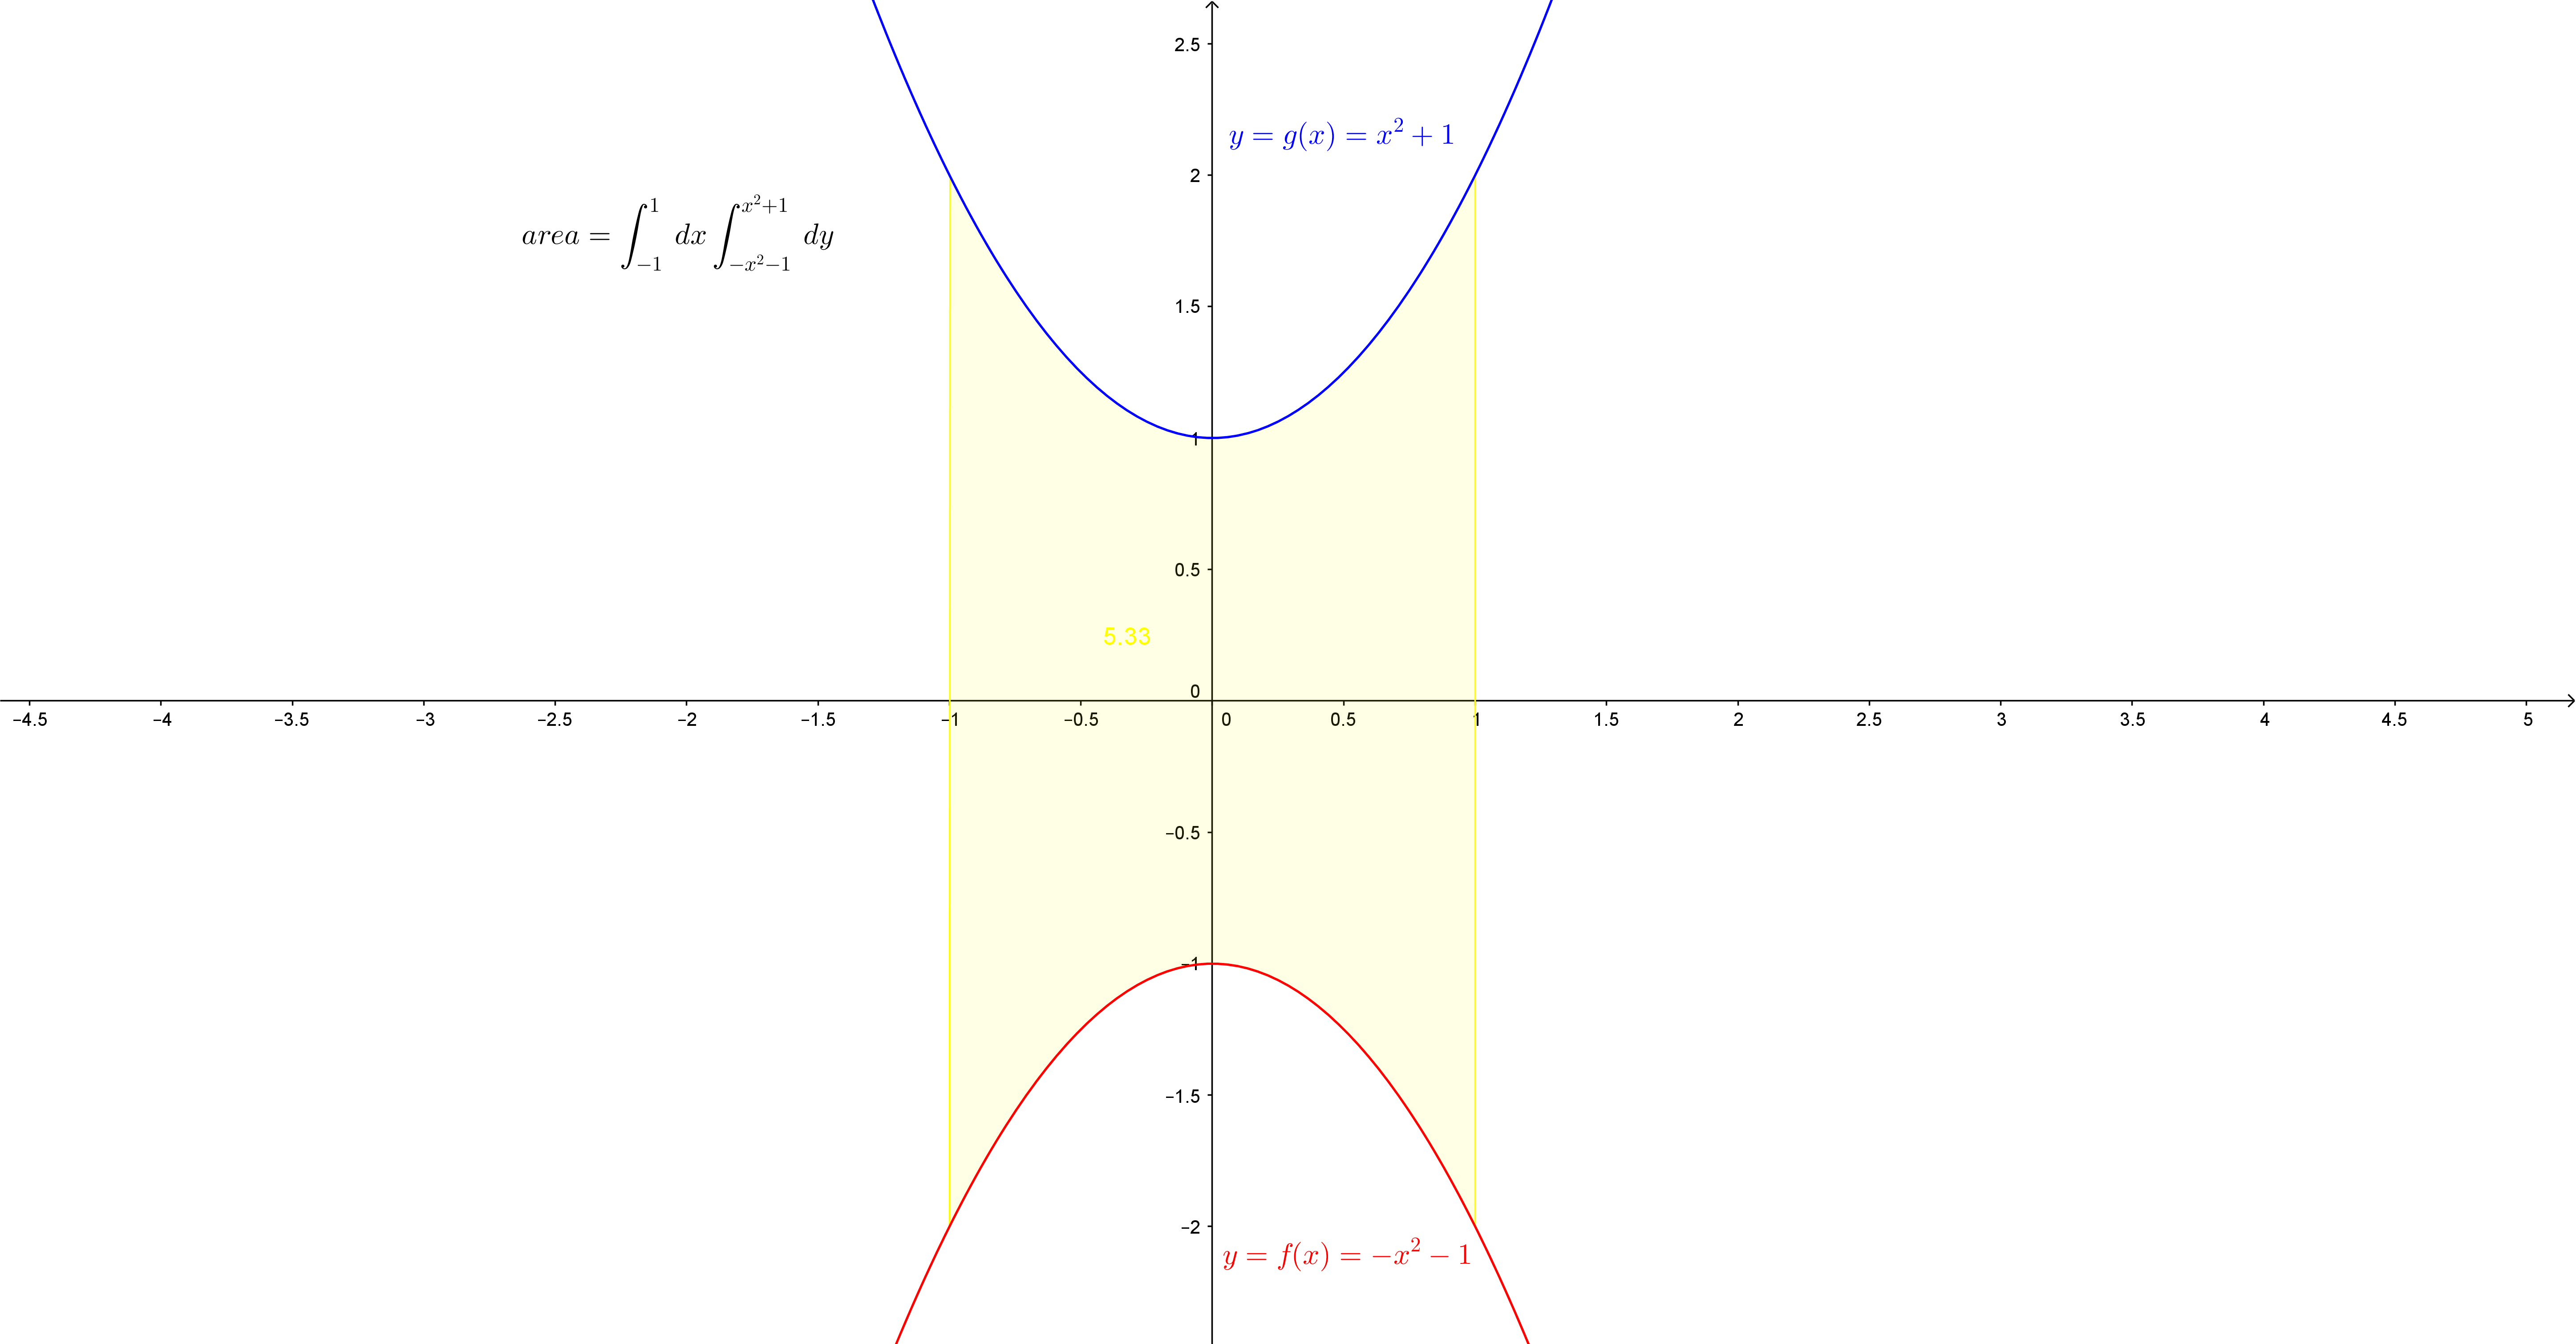
\includegraphics[width=0.5\textwidth]{v02_a02_e04.png}		
	\end{figure}
	
	\begin{gather*}
		a = \int_{-1}^1 dx \int_{f(x)}^{g(x)} dy = \int_{-1}^1 dx \int_{-x^2 - 1}^{x^2 + 1} dy = \int_{-1}^1 dx\, [y]_{-x^2 - 1}^{x^2 + 1} =\\ \int_{-1}^1 dx\, \left[x^2 + 1 - \left(-x^2 - 1\right)\right] = \int_{-1}^1 dx\, \left[x^2 + 1 + x^2 + 1\right] =\\ \int_{-1}^1 dx\, \left[2x^2 + 2\right] = 2\int_{-1}^1 x^2\, dx + 2\int_{-1}^1 dx = \left[2\dfrac{x^3}{3} +  2x\right]_{-1}^1 = \left[2\left(\dfrac{x^3 + 3x}{3}\right)\right]_{-1}^1 =\\ \dfrac{2}{3}\left[x\left(x^2 + 3\right)\right]_{-1}^1 = \dfrac{2}{3}\left[1 \cdot \left(1^2 + 3\right) - (-1)\left((-1)^2 + 3\right)\right] = \dfrac{2}{3}(4 + 4) = \dfrac{2}{3}8 = \dfrac{16}{3} = 5,\overline{3}	
	\end{gather*}
		
	\item Exercício
	
	\begin{equation*}
		R = \left\{(x, y) \in \mathbb{R}^2 \,|\, 0 \leq y \leq 2 \,,\, -y \leq x \leq y \right\}
	\end{equation*}
		
	\begin{figure}[htb]
		\caption{Integrais duplas - Aula 2 - Exercício V}
		\label{v02_a02_e05}
		\centering
		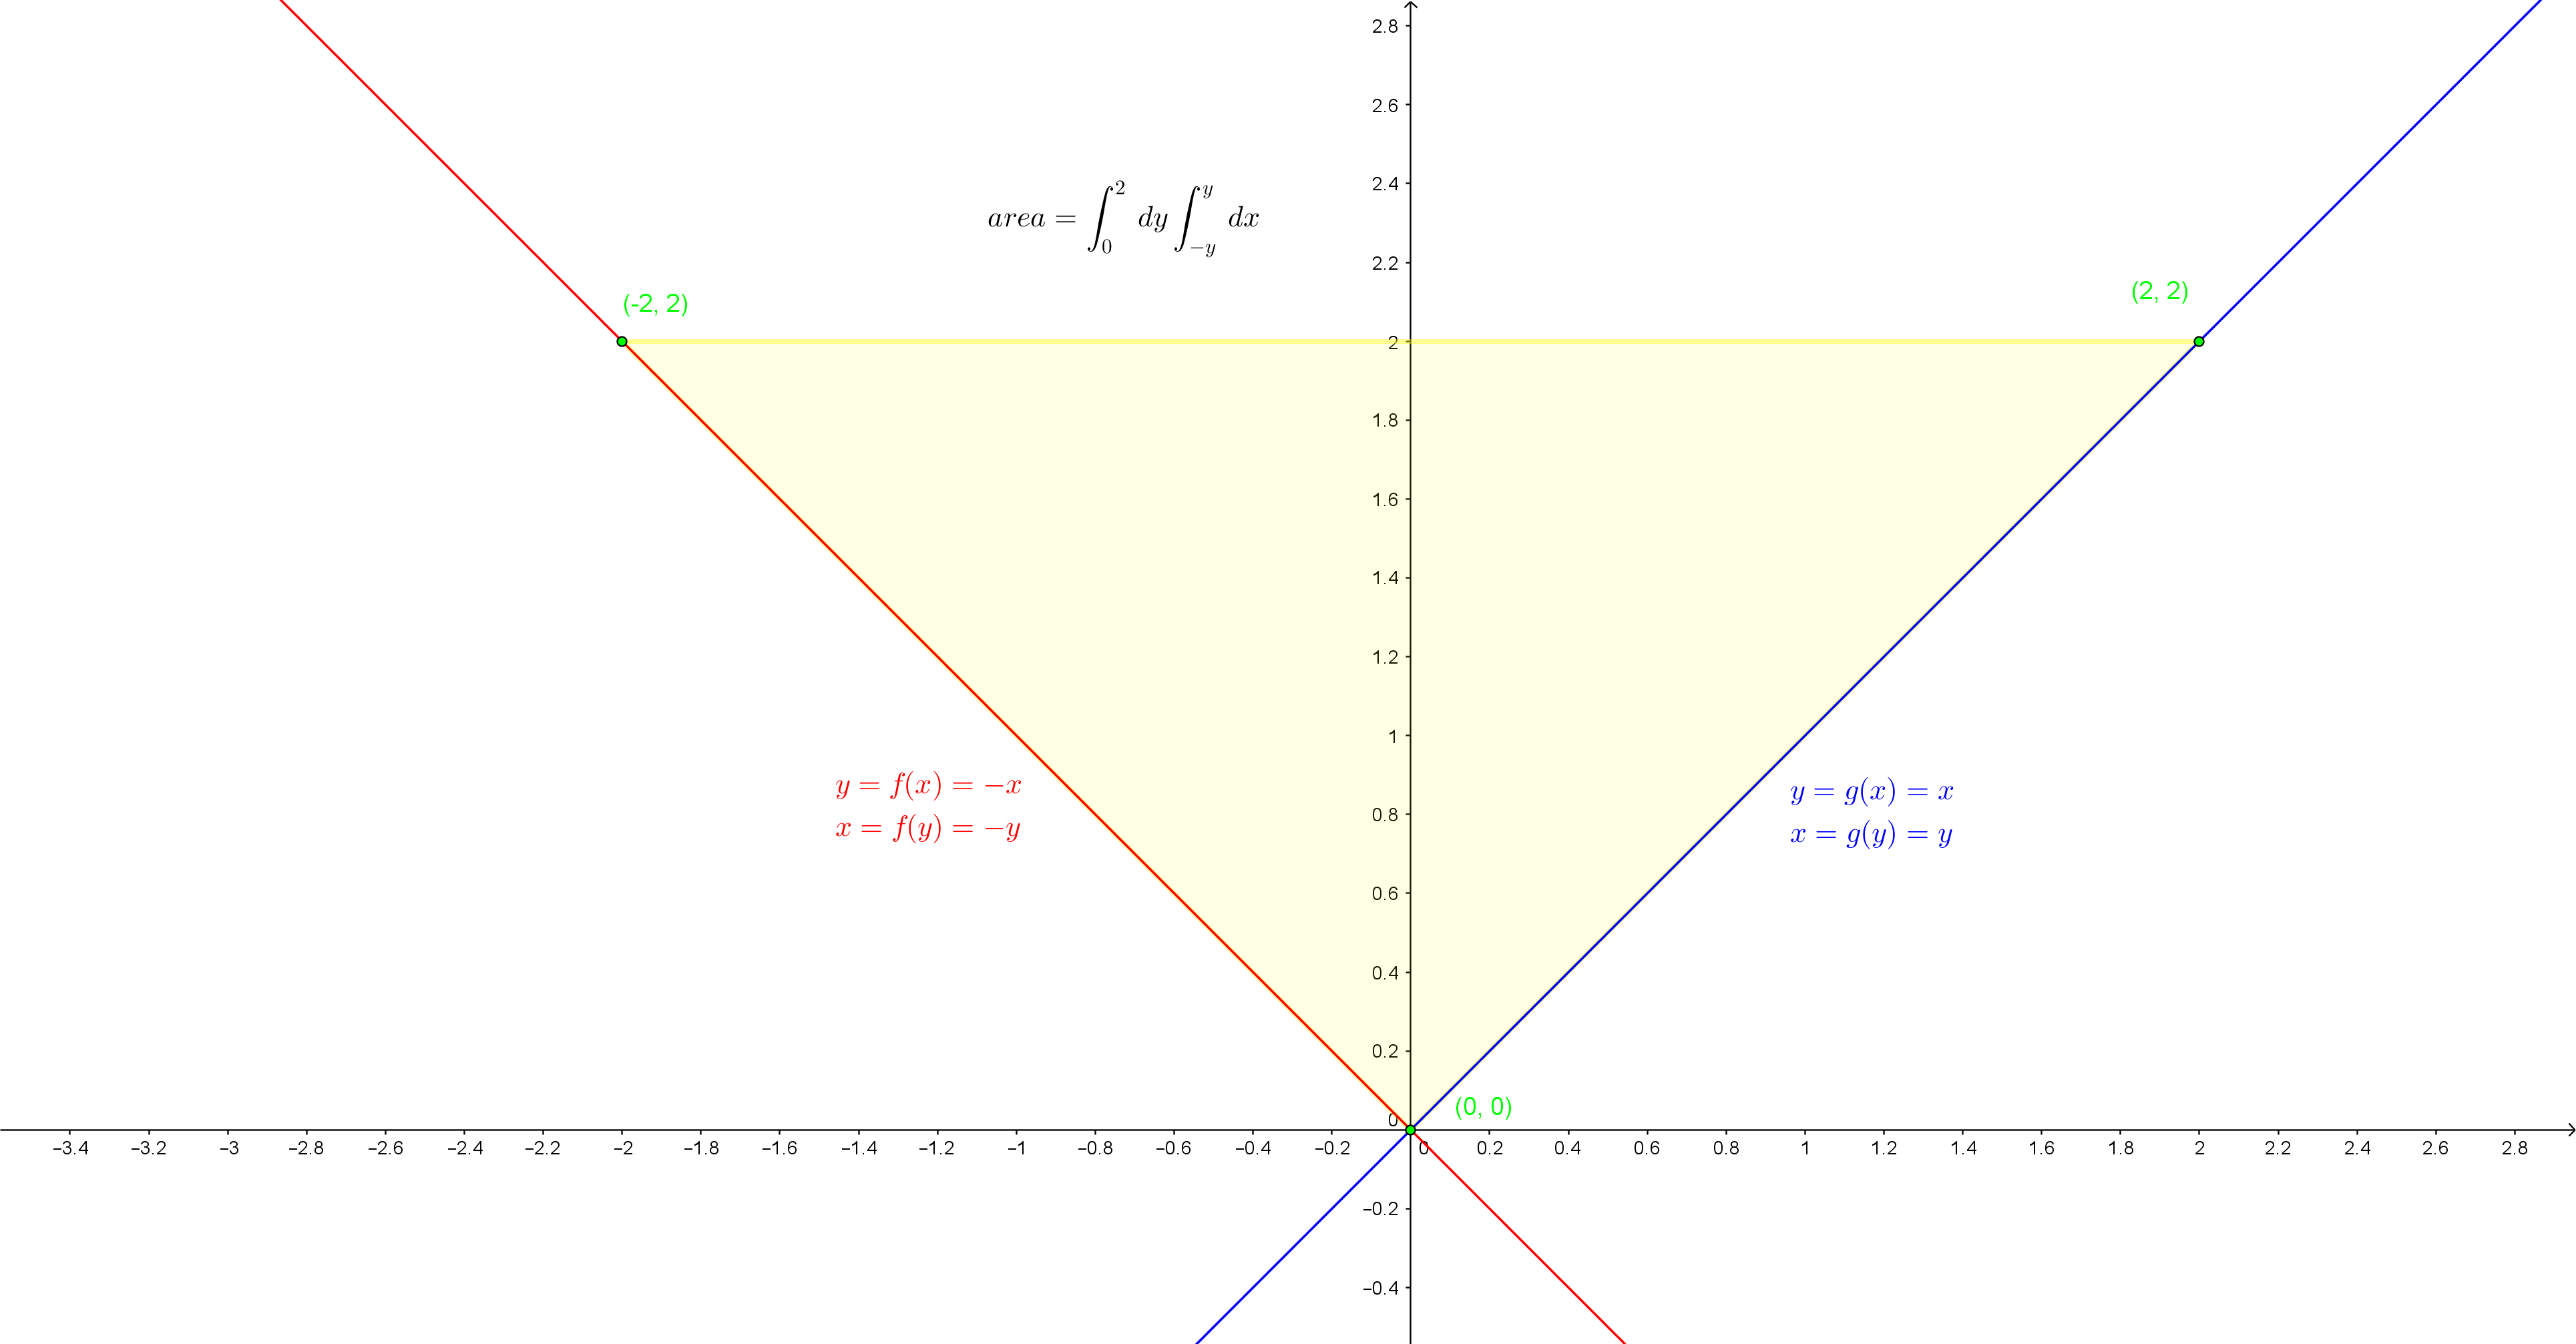
\includegraphics[width=0.5\textwidth]{v02_a02_e05.png}		
	\end{figure}
	
	\begin{gather*}
		a = \int_0^2 dy \int_{f(y)}^{g(y)} dx = \int_0^2 dy \int_{-y}^y dx = \int_0^2 dy\, [x]_{-y}^y = \int_0^2 dy\, [y - (-y)] = \int_0^2 dy\, [2y] =\\ 2\int_0^2 y\, dy = \left[\overstrike{2}\frac{y^2}{\overstrike{2}}\right]_0^2 = 2^2 - 0^2 = 4
	\end{gather*}
\end{enumerate}